\section{Apepndix}
\begin{figure}[H]
    \centering
    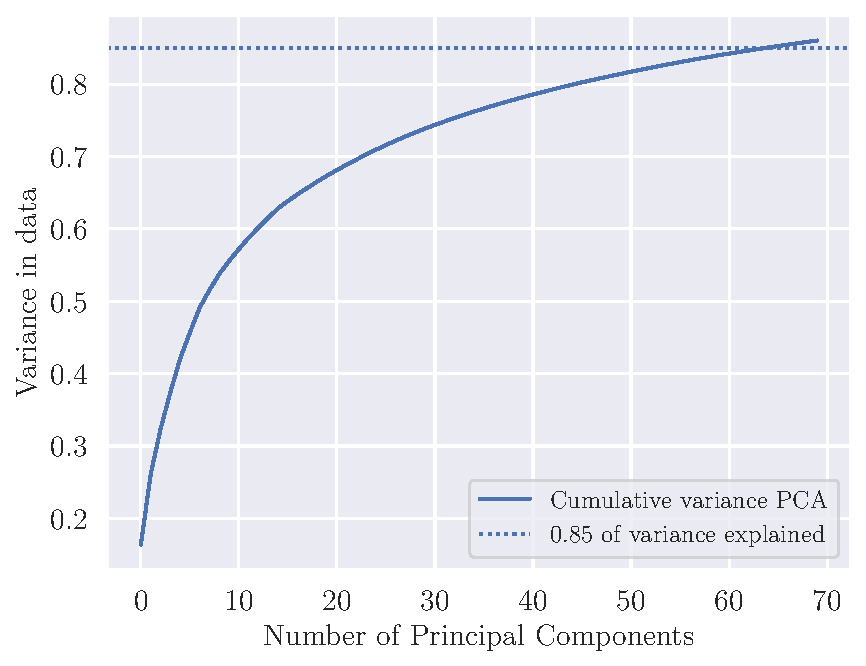
\includegraphics[width=0.9\linewidth]{examples/tests_eb/figs/cumsum_pca.pdf}
    \caption{A plot of the cumulative variance for each principle component included in our new, dimensionality reduced features. We concluded that 70 features was sufficient to capture just above 85 percent of the variance in our data.}
    \label{fig:cumsumpca}
\end{figure}

\begin{figure}[H]
    \centering
    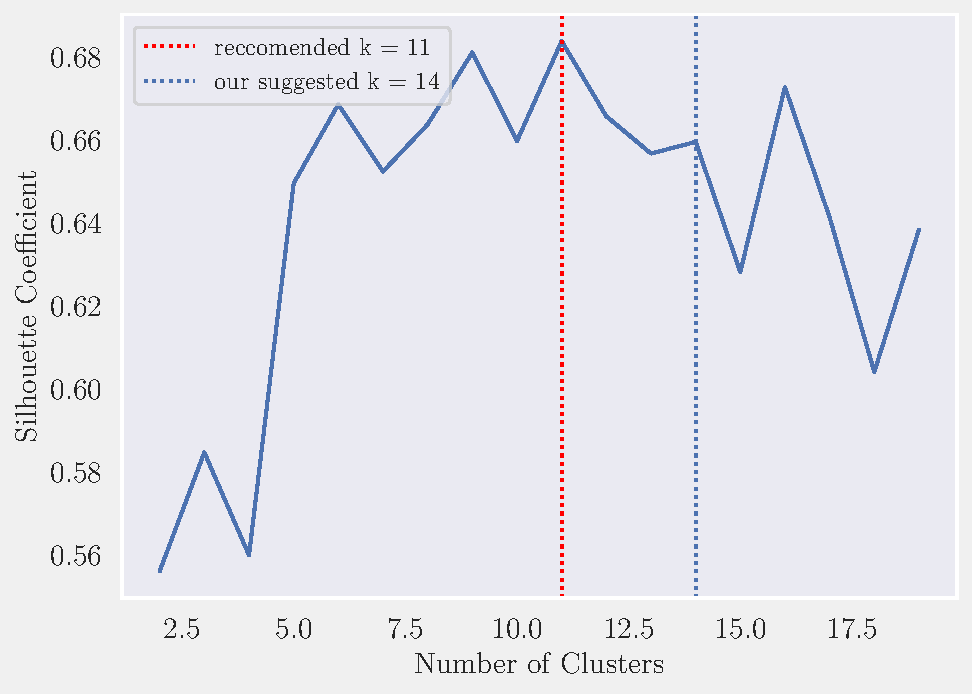
\includegraphics[width=0.9\linewidth]{examples/tests_eb/figs/kmean_sil.pdf}
    \caption{A plot of the silhouette scores for each KMean tested on UMAP data.}
    \label{fig_cumsumpca}
\end{figure}


\begin{figure}[H]
    \centering
    \begin{subfigure}[b]{1\linewidth}
        \includegraphics[width=\linewidth]{examples/tests_eb/figs/}
        \caption{Tintinnids-empty that have clustered with Pseudo-Nitzchia chains according to simple K-means clustering of an isolated selection of UMAP embeddings for the two species.}
    \end{subfigure}
    
    \vspace{1em}
    
    \begin{subfigure}[b]{1\linewidth}
        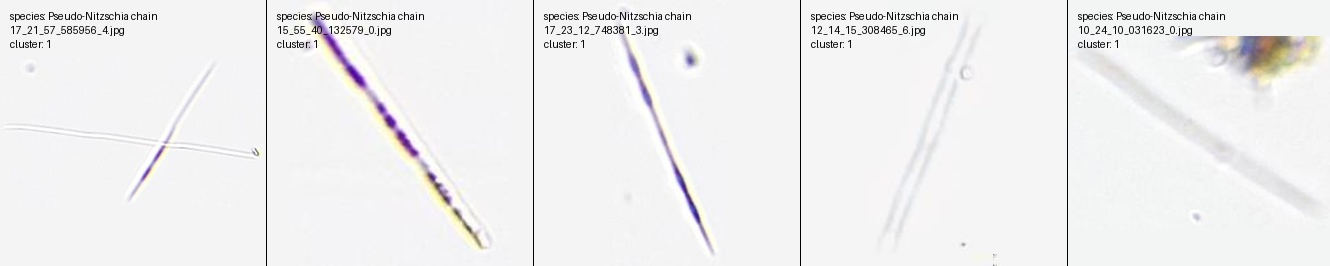
\includegraphics[width=\linewidth]{examples/tests_eb/figs/misclustered_pseudo-nitz.png}
        \caption{Pseudo-Nitzschia chains that have clustered with Tintinnids-empty according to simple K-means clustering of an isolated selection of UMAP embeddings for the two species.}
    \end{subfigure}
    \caption{We compare some of the species that seem to cluster together in Figure \ref{fig:umap} to explore whether the original labels are incorrect or if our DINOv2 fails to discern between the two species. The clustering process demonstrated in Figure \ref{fig:misclust_umap} and \ref{misclust_kmeansumap} in our Appendix.}
\end{figure}
